\documentclass[12pt,letterpaper]{article}
\usepackage{amsmath}
\usepackage{amssymb}
\usepackage[round]{natbib}
\usepackage[left =1.0in,right=1.0in,top=1.0in,bottom=1.0in]{geometry}
\usepackage{graphicx}


%opening
\title{}
\author{Xiaojuan Zhu}

\begin{document}

\maketitle

\begin{abstract}


\end{abstract}
%3) Outline for the paper.
%1. Introduction - What are the problems and key questions that you are trying to solve? How are you approaching it? What methods?  
%2. Literature review - What has been done before and published in academic or trade literature?  How have people discussed motivations for retirement and quitting in different industries.  What factors are in play?  How does solving this problem help companies?
%3. Data Description and Preparation
%4. Model Development and description
%5. Analysis of Modeling results
%6. Conclusions and managerial implications 
%If we can do 1,3,4,and 5 we may get Tim to help us with 2.

\section{Introduction}
Employee turnover is a topic that has drawn the attention of management researchers and practitioners for decades, because  employee turnover is both costly and disruptive to the functioning of most organizations \citep{staw1980, mueller1989,kacmar2006}, and both private firms and governments spend billions of dollars every year managing the issue according to \citet{leonard2001}. Therefore, understanding the causes of turnover: retirement and voluntary quit, examining the internal and external impacts, effectively forecasting the turnover by these two causes, and measuring the effectiveness and to what extent of the HR policy at firm and departmental levels are the key questions in this study for reducing it and for effective planning, budgeting, and recruiting in the human resource filed. As a funded research project, a large organizational secondary dataset including 12-year employees demographic information and records is transformed, analyzed and modeled by Cox proportional hazard regression models with a time dependent covariate using competing risks analysis to examine the statistically significant factors and to predict employees' conditional retiring and voluntary quitting probabilities. The dataset are also employed to logistic regression and time series models for compare the performance of cox proportional hazard model.This study also examines the forecasting capability of Cox proportional hazard model on the data with two kinds of bias (left truncation and right censor) by simulation.      


%Employee turnover cost impacts both the operational capabilities and the budget of an organization. The cost for turnover involves recruiting, selecting, training and developing \citep{mobley1982, staw1980}. According to the estimation from U.S. Department of Labor, turnover costs a company one third of a new hire's annual salary to 
%replace an employee, which is about \$500 to \$1500 per person for fast-food industry and \$3000 to \$5000 per person for trucking industry \citep{white1995}. Furthermore, turnover also disrupts the social and communication structures, and causes the productivity loss due to the replacement \citep{mobley1982}. Beyond the these cost and operational disruption, turnover demoralizes the attitudes of remaining employees and leads to additional turnover \citep{staw1980}. Therefore, understanding and forecasting turnover at firm and departmental levels is essential for reducing it \citep{kacmar2006} and for effective planning, budgeting, and recruiting in the human resource field. 

%this study is to forecast employee turnover in organizational level using time series and individual level using survival analysis, to examine the internal and external factors contributing on employee turnover, to identify why employee turnover, and to measure the effect of human resource policy on employee turnover based on employee demographic dataset. 

\section{Literature Review}
\section{Data Preparation}
%objective is to forecast employee retirement and voluntarily quit using statistical model\\
%1. data description \\
%a. The data is employee demographic information and records windows 10 years, data's detailed information. \\
The turnover dataset is a large real world secondary dataset from a multipurpose research organization in the U.S. The dataset consists 4316 current active and 3782 terminated full-time employees' information including metrics such as payroll category, hired date, company start date, company credit service date, termination date, age at hired , years of service at hired (YCSH), gender, job classification (named as Cocscode), and department code (named as division). The company credit service date is the date that the organization starts to credit their retirement plan. Years of service (YCS) is the total years credit for employees' retirement plan. The employees are eligible to get full retirement or pension, when their age is at least 65 or the points is greater than 85, which is the sum of age and year of service. The window of time for the turnover dataset is from November 2000 to December 2012, i.e. the dataset consists the records only for the employees working in the organization from November 2000 to December 2012, indicating there is no records for employees leaving the organization before November 2000 and no termination date for 4316 current employees. 

%b. data series plot and describe 2008 event.\\
%2. economic indicator variables, sources and what they are, why you select these economic index\\
Several economic indices are being considered and tested their as a variable impact on employee turnover. These indices include unemployment index, housing price index (HPI), investment index, and marketing index. Seasonal adjusted unemployment rate is published by Bureau of Labor Statics from United department of Labor \citep{unemployment}. U.S housing price index, U.S. and southeastern monthly purchase-only index are considered as another economic indicator variables in the study \citep{HPI}. S\&P 500 indices published from S\&P Dow Jones Indices are also considered as investment index including S\&P 500, Dividend, Earnings, Consumer index, Long Interest Rate, Real Price, Real Dividend, Real Earnings, P/E 10 ratio \citep{sp500}. Wilshire 5000 total market full cap index published by Wilshire Associates is considered as market index in the forecasting model\citep{will5000}. All these twelve indices are treated as variables using their twelve-month lag term in yearly data format. All these indices selected are indicators in various economic areas, such as job market, house market, and stock market, representing the fluctuation of these economic areas.    
%1. umployement indexm
%2. housing price indicator: s\&p case shiller  index   (us.s\&p.com)  monthly-only purchase index, monthly house price indexes for census division and US.
%3. investment index, s\&p500  finance.google 
%4. marketing index:  wilshire5000  total marketing  index
%5. NYSE code.

\section{Model Development and Description} 
\subsection{How to model employee turnover}
Several questions have to be addressed by this study, such as when a specific employee will turnover, how many employees will turnover in a curtain department or a job category, what factors do affect their turnover, by what reason they will turnover: voluntary quit or retirement. And also the dataset has two kinds of unknown information, which are no records for employees leaving the organization before November 2000 and no termination date for 4316 current employees. These two kinds of unknown information cause two kinds of bias: right censor and left truncation. Besides, there is an intervention event implemented in year 2008 due to the downsizing policy in the organization. Therefore, how to model this incentive and to estimate its effect are another interesting questions. All these questions and problems can be solved by lifetime analysis, also called survival analysis. The survival analysis is to analyze the time duration for the occurrence of an events or certain events. The events can be the death of the patients, the failure of the machine, and the leaving of the employees by any reasons for this study. There are two kinds of survival statistic models: parametric survival models and Cox proportional hazards (PH) models. In this study, Cox PH model is employed to build the forecasting model, to generate a employees' working life baseline (distribution), and to identify significant factors for turnover. The parametric models are not appropriate for this study, because it is hard to fit the employees' working life distribution to any parametric distributions, such as Weibull or log-normal distribution. Time dependent covariates are incorporated for fitting the 2008 intervention event due to the downsize policy in the organization and for examining the effects of economic indicators. Competing risks analysis is applied for modeling employee retirement and voluntary quit. Besides, A simulation study is performed to examine the forecasting capability of cox proportional hazard model on the left truncation and right censor dataset.
 %There are several reasons for employee leaving the organization: retirement, voluntary quit, layoff, transferring, leave of absence, or death. In this study, retirement and voluntary quit are selected and modelled respectively using competing risks analysis. 
 
 \subsubsection{Two data bias: right censor and left truncation}
 % what is right censor, how to deal with right censor\\
 % what is left truncation how to deal with left truncation\\
 Right censor and left truncation are common in survival analysis. The right censor is that the event of interest (failure) occurs after the study window.
 \begin{figure}[htbp]
 	\centering
 	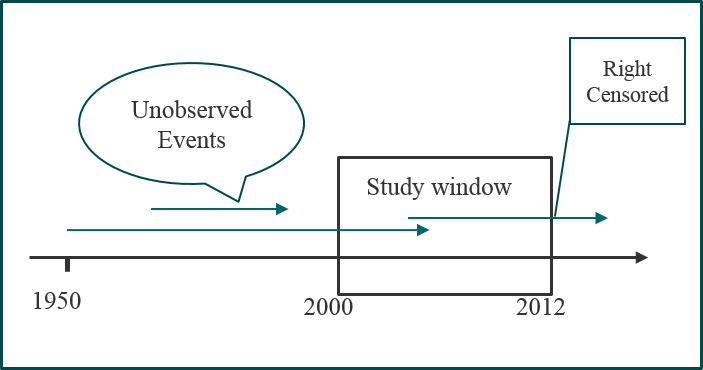
\includegraphics[width=3.5in]{fig1.png}
 	\caption{Right censor and left truncation}
 	\label{fig:1}
 \end{figure}
  Let $T$ denotes the time of main event of interest to occur and let $C$ denotes the end time of study. An observation is right censored when $T> C$, indicating the study do not have the failure time of the right censored observation. In this study, the study window is from November 2000 to December 2012 as shown in the figure \ref{fig:1}. Thus, the current active employees have unknown terminated date. They are treated as right censor. These right censored observations require special treatment in survival analysis: a censor indicator variable is created: 
 \begin{align*}
 	\delta_i&=
 	\begin{cases}
 		1   &\text{if  }  t_i \leq c_i \text{ (uncensored),}\\
 		0   &\text{if  }  t_i > c_i \text{ (censored),}
 	\end{cases}
 \end{align*}
 where, $i$ denotes the ith observation, and the failure time of event for ith observation is minimum time between $t_i$ and $c_i$, i.e., $min(t_i, c_i)$, that is when $ c_i <t_i $, $c_i$ is taken as end time of the ith observation in order to do next  analysis.
 
 Left truncation is that the occurrence of an intermediate event prior to the event of interest appear in the sample dataset. Let $T$ denotes the time of event of interest to occur and let $X$ denotes the time an individual enters the study, that is time of truncation events occurs. Only the individuals with $T \geq X$ are observed in the study window. Left truncation in this study occurs due to no records for employees leaving the organization before November 2000 as unobserved events shown in the figure \ref{fig:1}. The left truncation leads to another bias. As shown in the figure \ref{fig:1}, the longest arrow represents a life time for an employee hired in 1950 and left in 2006. Those employees who remain in the study window increase the apparent lifetimes. The existence of truncation in the data must be taken into account in order to overcome this bias and to achieve accurate estimation of survival analysis \citep{carrion2010}. Let $t_{i0}$ denotes the start time of the ith observation, i.e., hired time or age at hired of ith employee, $x_{i}$ denotes the entry time of the ith observation, i.e., the start time of study (November 1st, 2000) or age at November 1st, 2000. The start time of the observation is maximum value between $t_{i0}$ and $x_i$, that is when $t_{i0} < x_i $, $x_i$ is taken as start time of the ith observation in order to eliminate the left truncation bias \citep{allison1995}. The number of failures in the $t_j$ is redefined for left truncation. When $x_i < t_j \le t_i$, the observation is in the risk set. When $t_{j} < x_i \le t_i$, the ith observation has not entered study yet at $t_j$ and it cannot be considered in the risk set. When $x_i \le t_i < t_j$, it indicates the ith observation whose failure time before $t_j$, and it cannot be considered in the risk set at time $t_j$ neither \citep{carrion2010}.
 
 simulation study.

\subsubsection{Cox ph regression model}
%   1. what is cox ph regression model.

Cox proportional hazards (PH) regression is a widely used method for estimating survival life events, introduced in a seminal paper by \citet{cox1972}. The Cox PH model is usually taken the form of hazard model formula as shown in the equation \ref{eq:cox}:
   \begin{equation}
   \label{eq:cox}
   h(t,x)=h_0(t)e^{(\sum_{i=1}^{k}\beta_ix_i)}
   \end{equation}
   
   where $x=(x_1, x_2, \ldots, x_k)$, $h_0(t)$ is the baseline hazard occurring when $x=0$, $\beta$ is the coefficients of $x$. 
%    why not parametric. baseline cannot fit to any parametric model\\
%    2. cox regression without/ with time dependent variable\\
   The model provides a hazard expression at time t for an individual with a given specification of a set of explanatory variables denoted by the $x$. The Cox PH formula is the product of quantities at hazard time $t$: $h_0 (t)$ as the baseline hazard function and the exponential expression to the linear combination of $\beta_i x_i$, $x$ does not involve time $t$, so it is time-independent covariates. $x$ can also be time-dependent covariates, which named extended Cox PH regression as discussed in the section \ref{sec:coxt}. 
   The Cox PH regression is "robust" and popular, because the baseline hazard function $h_0 (t)$ is an unspecified function and its estimation can closely approximate correct parametric model \citep{kleinbaum1998}. Taking the logarithm of both sides of the equation, the Cox PH model is rewritten in the equation \ref{eq:coxlog}:
   \begin{equation}
   \label{eq:coxlog}
   \log{h(t,x)}=\alpha(t)+\sum_{i=1}^{k}\beta_ix_i 
   \end{equation}
   where $\alpha(t)=\log{h_0(t)}$. If $\alpha(t)=\alpha$, the baseline is exponential distribution. In the Cox PH regression, $\alpha(t)$ do not limited on specific parametric distributions and it can take any form. The partial likelihood method is used to estimated $\beta$ coefficients of the Cox model without having to specify the baseline \citep{allison1995}.
  
 
\subsubsection{Time dependent covariate and counting process}
\label{sec:coxt}
A time dependent covariate is that a covariate is not constant through the whole study and its value changes over the course of the study. The extended Cox PH regression model incorporates both time-independent and time-dependent covariates as shown in the equation \ref{eq:timecovar}:
\begin{equation}
\label{eq:timecovar}
h(t,x)=h_0(t)e^{(\sum_{i=1}^{k_1}\beta_ix_i+\sum_{j=1}^{k_2}\gamma_jx_j(t))}
\end{equation}
where $x=(x_1, x_2, \ldots, x_{k_1}, x_1(t), x_2(t), \ldots, x_{k_2}(t))$, $h_0(t)$ is the baseline hazard occurring when $x=0$, $\beta$ and $\gamma$ are the coefficients of $x$. 

    I. due to 2008 intervention, each employee have different age at 2008, we have use counting process. Each employee has up to 3 records related to the time, which is before 2008, in-between 2008, and after 2008. The variables related to time are changed based on years, such as policy, age, year of service. Policy is a dummy variable in the form as shown in equations. 
    Two age points are calculated for each record at each period: one is age at beginning of the certain period, named "age at start"; and the other one is age at end of the curtain period, named "age at end".
    Two year of services variables are also generated for each record at each period: one is year of service at the beginning at the period, named "YCS at start"; the other one is the year of service at the end of the period, named "YCS at end".\\
    II. economic indiecators, is time dependent external variables, we have split each employee's the record into yearly records, so each employee has up to 12 records.  
    What is counting process.   \\ 

\subsubsection{Competing risks}
  what is competing risks. competing ricks can help forecasting employee retirement and voluntary quit. \\
  why select these two reasons to model.\\
\subsubsection{Stratification model}
  I. what is stratification model;\\
  II. how to select a stratify variable\\
\subsubsection{Variable selection}
 all the variables are putting into model and selected by backwards selection methods based on P-value.\\
\subsection{Model validation and comparison}
\subsubsection{Measurements}
 AIC, BIC, MAPE, c statistic.\\
\subsubsection{Model validation}
 1. Forecast employee turnover   how to forecast and calculate employee turnover number\\
 2. conditional probability (The prediction is conditional probability): given the employee is survival at last year, what is the probability they survival or quit for this year.\\
 3. the total number of employee turnover is the aggregate all turnover probabilities of employees at each year\\
      
 4. split data into two ways: both training and holdout, training to build the model and holdout is to validate the model, and compare the actual vs forecasting, calculated MAPE and C statistics. \\ 
       WAY1: training (10 years)and holdout (2 years). forecasting the total number of employee leaving the organization, compared to the actual number to calculate MAPE and C statistics. compare to logistic regression and time series methods to shown survival is better.\\
       WAY2: random split the data into training (2/3) and holdout (1/3), using c statistics to select one best survival model.
  
\subsection{Results}
\subsubsection{Right censor and left truncation simulation results}
\subsubsection{Retirement model without external variables}
   1. four survival model have been generated for comparison. 
   2. significant variables.
   3. stratfication variable deterimation.
   4. model comparison based on validation way 1 and way2 (one table show all the models) 
\subsubsection{Retirement model with external variables}
     best model and tested which variable does significantly impact on retirement.
\subsubsection{Voluntary quit model without external variables}   
     I. dependent variable are YCSH, because age is not able to predict well.
     II. shorten the length of risk set.
     iii. model comparison. (survival model, time seris model, and logsitic regression model)
\subsubsection{Voluntary quit model with external variables}
    i. tested which variable does significantly impact on employee voluntary quit.
     

\section{Conclusions and Managerial Implications} 


	\bibliographystyle{abbrvnat}%Choose a bibliograhpic style%
	\bibliography{Bib}
\end{document}
